\documentclass[conference, a4paper]{IEEEtran}

\usepackage{graphicx}

\graphicspath{{./images/}}

\title{Anomaly Detection Using Machine Learning Techniques for Beam Injections from the SPS to the LHC at CERN}
\author{\IEEEauthorblockN{Marc Ferriggi}
	\IEEEauthorblockA{Department of Computer Science\\
	Faculty of ICT\\
	University of Malta}
	\and
	\IEEEauthorblockN{Dr Ing. Gianluca Valentino}
	\IEEEauthorblockA{(Supervisor)\\
		Faculty of ICT\\
		University of Malta}
}
\IEEEspecialpapernotice{(Review Paper)}

\begin{document}
	\maketitle
	\begin{abstract}
		Filling the LHC is a challenging task and anomalous injections are common when operating such a large machine. In this dissertation, unsupervised machine learning techniques for anomaly detection were used to analyse past data in order to understand the sources of the anomalies for improving the LHC machine availability and performance reach. Data from sensors around the moment of injection from the SPS to the LHC were analysed and different feature sets were chosen as input parameters for the anomaly detection algorithms. In this study, LOF was found to achieve the best performance when run on the full feature dataset with an accuracy of 92.76\% for Beam 1 and 91.08\% for Beam 2. The anomalous points are also visualised in 3D plots which serve to help researchers understand better the nature of these anomalies. Furthermore, the beam's position drift with time is also presented and is shown to also be a factor in impacting the injection quality.
	\end{abstract}

	\section{Introduction}
	\par The Large Hadron Collider (LHC) is a two-ring superconducting hadron accelerator and Collider installed at the CERN and commenced operation in 2008 \cite{Evans2008}. The Collider is 26.7km long and its purpose is to accelerate and collide two heavy ion beams \cite{Valentino2017}.
	
	\par In order to operate the LHC with a centre-of-mass energy of 14 TeV, twelve injections from the Super Proton Synchrotron (SPS) consisting of a number of proton bunches of around 1 MJ of stored energy are required \cite{Drosdal2011}. Thus, in order to fill the LHC, approximately 4 minutes per beam is required. Furthermore, the whole experiment process of filling the LHC, performing the required checks, running the tests and dumping the beam should take a theoretical minimum of 70 minutes \cite{Evans2008}. However, from past experiences, this is expected to take longer, partly due to unsuccessful or anomalous proton injections to the LHC. 
	
	\par Clearly, filling the LHC is a challenging task given the high energy of the beam, the very small apertures and the delivery precision's tight tolerances. The beam must pass through many accelerators and transfer lines before reaching the LHC. During this process the beam must be monitored, thus multiple sensors are installed around the CERN particle accelerator complex \cite{Lefevre2008} which gather readings and data that can be used to check the quality of the injected beam. 
	
	%%Establishing a Niche:
	\par For this particular study, data generated from the sensors around the injection from the SPS to the LHC will be of particular interest. As the first beam (Beam 1) leaves the SPS, it must pass through the transfer line TI2, while the second beam (Beam 2) must pass through TI8. The data from sensors around these transfer lines as well as at some points around the LHC and SPS will be used in this study and are stored using CERN's Logging Service (LS) \cite{Roderick2013}. While many studies have been made using this logged data and lots of statistical tests have been done with regards to injection quality checks for the LHC (such as \cite{Drosdal2011} and \cite{Kain2010}), no literature was uncovered where researchers used unsupervised machine learning methods to analyse this particular data.
	
	\par Furthermore, the Injection Quality Check (IQC) software currently installed has a set of hard-coded rules for detecting anomalies in the SPS-LHC injection \cite{Drosdal2011}, however there are documented cases in the past where situations occurred which were outside the originally foreseen rules and were therefore not caught as anomalies. Apart from causing experiments to fail, these anomalous injections could be very costly as a lot of data must be examined after such failures which wastes time that could be used to run more experiments \cite{Halilovic2018}. 
	
	\par The major cause of these anomalies is due to the fact that the machine is so large, and needs to be so precise, that minor ground motions over time affect the tilts in the quadrupole magnets which thus affect the orbit of the beam. Figure \ref{fig::AnomalousInjections} highlights two possible cases of anomalous injections. The first case shows what happens to the beam when the Beam Position Monitor (BPM) gives a high Mean Square Error (MSE) reading with respect to its original position in the first injection of the season. The second case shows what happens to the beam when there is a high loss recorded by the Beam Absorber for Injection (TDI) Beam Loss Monitors (BLM).
	
	\begin{figure}[!t]
		\centering
		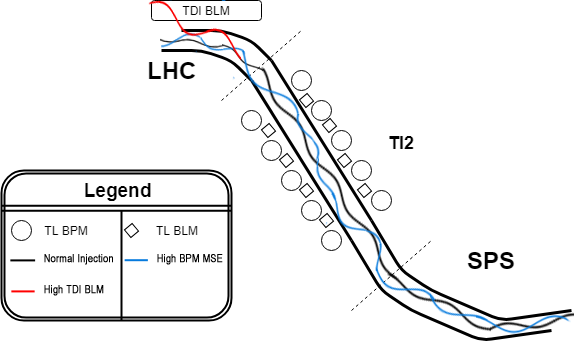
\includegraphics[width=2.5in]{AnomalousInjections}
		\caption[Anomalous Injections]{Examples of Anomalous Beam Injections showing the locations of the BPMs and BLMs in the transfer line}
		\label{fig::AnomalousInjections}
	\end{figure}

	\par The purpose of this study is to apply unsupervised anomaly detection algorithms to try solve the problem of detecting anomalous injections with the hopes of finding a technique that will detect the anomalies not being picked up by the IQC. This can help researchers understand the source of these anomalies and improve the LHC machine availability and performance reach in terms of beam lifetime, beam stability and luminosity.
	
	\par In Section 2, the background to the problem domain is explained in further detail with the intention of providing the reader with information needed to fully understand this study. The methodology used to analyse the provided dataset can be found in Section 3 where work done on the entire data science process is presented. The results of this study are then presented in Section 4 and a detailed evaluation on the performance of the anomaly detection algorithms can be found in Section 5. Some final conclusions and suggestions for further work are then presented in Section 6.
	
	\section{Background}

	\par This section describes the different types of sensors that were used to collect the data, highlighting the particular details which need to be considered when analysing this data.
	
	%BLMs & TDI BLMs
	\par The BLMs are some of the most safety critical modules of the LHC because a loss of a very small fraction of this beam may damage parts of the machine or cause a quench in the superconducting magnets \cite{Holzer2006}. A high beam loss reading could also indicate over-injection. In fact, an injection of a high intensity beam into the LHC is only allowed if there is a low intensity bunch circulating the LHC in order to avoid settings errors \cite{Kain2010}. The BLM module is the mostly used module in the current IQC software checks \cite{Drosdal2011}. The BLMs must be reliable; the probability of not detecting a dangerous loss was found to be $5\times10^{-6}$ Gy/s per channel and they are only expected to generate 20 false dumps per year \cite{Holzer2006}. The BLMs are extensively logged to a database for offline analysis \cite{Holzer2006}. 
	
	%BPMs
	\par The BPMs were installed as a system for fast monitoring of the beam's position with respect to its orbit drift \cite{Schmidt2006}. The trajectory offsets recorded by the BPMs in the transfer lines must be minimised in order to reduce losses \cite{Drosdal2011}. In fact, if the change in orbit substantially exceeds its provided boundary values then the beam should be dumped \cite{Schmidt2006} so as to not cause any damage to the equipment.
	
	%Abort Gap
	\par When filling the LHC, it is necessary to keep an abort gap (i.e. an absence of particles) of at least 3$\mu s$ (each turn of the LHC is $\approx87\mu s$ long) in order to accommodate for the horizontally deflecting extraction kicker magnets (MKD) rise time \cite{Meddahi2010}. As the LHC is filling to nominal intensity, this gap will be populated with un-trapped particles and particles leaking out of their Radio Frequency (RF) buckets \cite{Meddahi2010}. The Abort Gap Monitor (AGM) was hence specifically designed to measure this particle population in the abort gap \cite{Lefevre2010}.
	
	%SPS and LHC Intensities
	\par The actual intensities of the circulating beam are measured by Beam Current Transformers (BCT). For the LHC in particular, a fast BCT is used which is capable of monitoring a broad range of currents as it must be able to detect a single pilot bunch circulating the machine (of 10 $\mu$A) as well as the full nominal machine (over 0.5 mA) \cite{Jones2007}. These readings are then converted from amps to number of protons per beam and stored for analysis. 
	
	
%	\section{Anomaly Detection in Particle Accelerators}
%	
%	\par In the paper released entitled ``Opportunities in Machine Learning for Particle Accelerators'' \cite{Edelen2018}, it was stated that due to the ``large number of process variables, non-linear behaviour, and many interacting subsystems,'' conventional analysis techniques on today's particle accelerator data is often insufficient and thus machine learning could be used as a means of anomaly detection. Furthermore, the authors also stated that these techniques could be used to ``identify and throw away bad signals.''
	
%	\par In his Master's Thesis, A. Halilovic used anomaly detection techniques solely on data obtained from the injection kicker magnets \cite{Halilovic2018}. Halilovic made use of a Gaussian Mixture Model and Isolation Forests to detect anomalies however found that the best performance achieved by his proposed pipeline ``leaves something to be desired'' as too many anomalies were not correctly classified. The author also goes on to suggest that analysing LHC data using the LOF class provided in `\textit{scikit-learn}' could lead to interesting results.
	
	%\par Wielgosz, \textit{et. al.} also wrote a scientific paper on using anomaly detection techniques on the LHC magnets \cite{Wielgosz2017}. This time, the authors went for a supervised approach and used Recurrent Neural Networks. They found that using adaptive quantisation to reduce 20-bit inputs into a 4-bit representation was an essential step in improving the algorithm's performance. The authors also stated that these anomaly detection techniques being proposed should not only be considered useful for CERN equipment but also useful in the broader field of anomaly detection on time series data.
	
	%\par In 2017, Valentino \textit{et. al.} released a paper on using anomaly detection techniques ``to detect minor changes in the loss maps over time due to collimator settings errors or orbit variations'' \cite{Valentino2017}. The authors used PCA as a dimension reduction technique and then applied LOF on the resulting 2 dimensional data. Their proposed method was shown to positively identify these anomalous loss maps based solely on BPM and BLM readings. Furthermore, they proposed using this technique to monitor losses during fills of the LHC.

	\section{Methodology}
	
	\subsection{Data Collection}
	\par The data used in this study was collected from the user interface to the LS (TIMBER) with the help of Dr Ing. Gianluca Valentino who has access to the CERN Intranet. Data was collected from the instrumentation discussed and covers 1624 Injections over a time period of 3 months (from 17\textsuperscript{th} August to 20\textsuperscript{th} October 2018). During this time, approximately 65 LHC fills were performed.
	
	\subsection{Data Cleaning and Analysis}
	\label{sec::Data_Cleaning_and_Analysis}
	\par After Data Extraction, the provided datasets were analysed separately in order to understand their nature, remove any outliers and be able to aggregate the data correctly for further analysis. In this section the results of this analysis will be presented with the hopes that the reader will have a clearer understanding of later results. Note that all the steps mentioned here were repeated for both beams.

		\begin{figure}[!b]
		\centering
		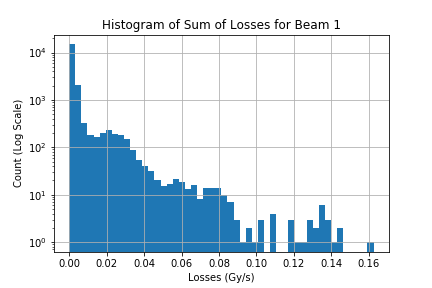
\includegraphics[width=2.5in]{Histogram_of_Sum_of_Beam_Losses}
		\caption[BLM Histogram]{Histogram of Sum of Losses for Beam 1}
		\label{fig::TDI_BLM_hist}
	\end{figure}

	\paragraph{TDI BLMs}There are three BLMs in the TDI, each one giving 10 readings around the moment of injection. In order to get a total loss for each injection, the sum of each reading from the 3 monitors was taken (Figure \ref{fig::TDI_BLM_hist}). It was noted that at the exact moment of injection, there was a spike in the amount of beam lost, thus in order to then obtain a single reading corresponding to that particular injection, the maximum sum of losses for each 10 second window was kept. Once the relevant readings were kept, the sum column was dropped and this data set was saved to be used for anomaly detection. Furthermore, after scaling these points using MinMax scaling, it was noted that the readings from the 3 monitors are highly correlated. This was confirmed by computing the correlation matrix which gave a Pearson Correlation value $> 0.98$ for all pairwise comparisons. 
	
	
	
	\paragraph{Abort Gap}The change in Abort Gap population is of interest for this study, thus the difference between every 10\textsuperscript{th} reading was kept and saved to be used for anomaly detection. Figure \ref{fig::Change_in_Abort_Gap_hist} shows the histogram of the Change in Abort Gap Population.
	
	\begin{figure}[!t]
		\centering
		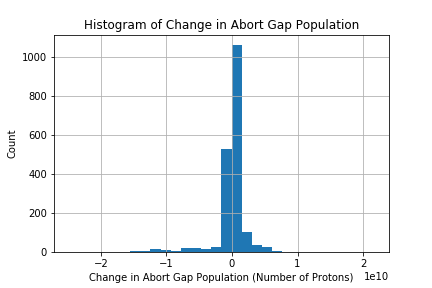
\includegraphics[width=2.5in]{Histogram_of_Change_in_Abort_Gap_Population}
		\caption[Change in Abort Gap Histogram]{Histogram of Change in Abort Gap Population for Beam 1}
		\label{fig::Change_in_Abort_Gap_hist}
	\end{figure}

	\paragraph{SPS and LHC Intensities}It is expected that change in LHC intensity at the moment of injection (10\textsuperscript{th} reading - 1\textsuperscript{st} reading) should be approximately equal to the SPS intensity value. Some of the beam however is lost in the transfer line (which is picked up by the TL BLMs) and as it enters the LHC (which is picked up by the TDI BLMs). Thus as an input parameter to the anomaly detection algorithm, the change in LHC intensities and the SPS intensities were extracted for each injection and saved. Figure \ref{fig::SPS_and_LHC} shows the increase in the LHC reading and the corresponding SPS intensity.

	\begin{figure}[!b]
		\centering
		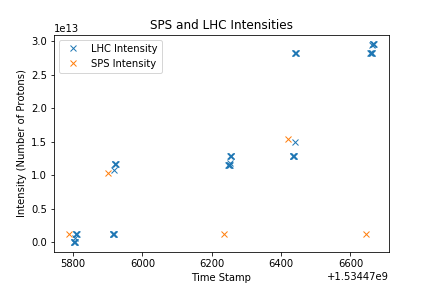
\includegraphics[width=2.5in]{SPS_and_LHC_Intensities}
		\caption[SPS and LHC Intensities]{Time Series of SPS and LHC Intensities for the first 5 Injections for Beam 1}
		\label{fig::SPS_and_LHC}
	\end{figure} 

	\paragraph{TL BLMs}Each TL has 61 BLMs each recording the amount of losses separately. The issue with these readings however is that their readings are not consistently stored after the experiments have been performed. In fact, during the time of the study, 13 of these monitors didn't have any logged data at all. The data which was logged was either 0 or close to 0. Thus, it was decided to drop this feature from the study.   
	
	\paragraph{TL BPMs}There are 18 BPMs in each TL, each one giving a separate reading of the beam's deviation from its expected path at a different position in the TL. From data taken from 1624 injections, data corresponding to 1420 injections was left for Beam 1 after removing all missing values and 1455 injections for Beam 2. Figure \ref{fig::BPM_hist} shows the histogram of the readings recorded by the first monitor in TI2. In order to measure the beam drift over time, the first injection was assumed to be the expected path and the MSE of each injection with respect to the first injection was taken. The first injection was used as the ideal expected path of the beam and any drift from this path would result in possible anomalous injections. This was worked out by taking the average of the squared differences in the readings of each monitor for each injection.
	
	\begin{figure}[!t]
		\centering
		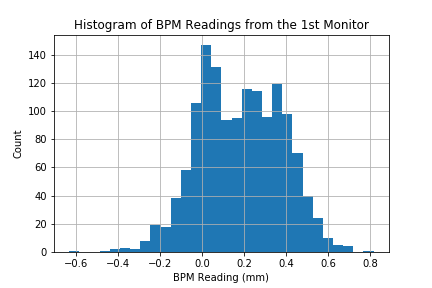
\includegraphics[width=2.5in]{Histogram_of_BPM}
		\caption[BPM Histogram]{Histogram of the readings recorded by the first monitor in TI2}
		\label{fig::BPM_hist}
	\end{figure} 

	\paragraph{Number of Bunches}The number of bunches injected into the LHC was another useful feature that needed to be extracted for normalisation. The beam losses, change in intensities and change in abort gap population are all relative to the number of bunches injected into the LHC as for example, a large loss may only appear to be large because more bunches were injected into the LHC for that injection than previous injections. In this case, that large loss should not be considered an anomaly. After the first single bunch is injected, the number of bunches injected in one go are typically multiples of 12, e.g. 12, 96, 144 which derives from how they are set up in the injector accelerators. The number of bunches circulating the LHC was hence extracted around the time of each injection and the change in number of bunches was then worked out.
	
	\subsection{Feature Selection}
	\par Two datasets where extracted for this study; a three dimensional dataset and the `full' dataset. One of the TDI BLMs, the change in LHC intensity minus the SPS intensity (i.e. the amount of beam intensity lost in the transfer line) and the MSE of the BPM readings were chosen as the three dimensional features. When performing the study on the `full' set of data, once again only one of the 3 TDI BLM readings would be needed as a feature. Furthermore, the readings from the TL BLMs were not used. Thus, the total number of dimensions used in the full model was 21 dimensions. Note that all readings were appropriately normalised by the number of bunches.

	\subsection{Anomaly Detection}

	\par After all the data cleaning and preparation, the resultant consistent data was ready to be used for anomaly detection. Each feature was first scaled using standard scaling. LOF and DBSCAN were then run for both Beam 1 and Beam 2 given this scaled and normalised data. PCA was also performed on the full-feature dataset and it was chosen to keep the components that explain at least 80\% of the data's variation, leaving 5 components for both Beam 1 and Beam 2. LOF was then performed on this resultant dataset.
	
	%% Paragraph on choosing the LOF and DBSCAN Parameters 
	\par When fitting the algorithms, care was taken to ensure the correct parameters were used in the models. Since this is an unsupervised approach, fitting the correct parameters is crucial to the overall performance of anomaly detection algorithms. However, since we do not have any training sets or guidelines on what points are actual anomalies, the parameters were tweaked by visual inspection of the resultant 3D plots derived after running the algorithm. In order to compare the performance of the different algorithms, the anomalous points detected were then manually checked on TIMBER by Dr Ing. Valentino and labelled accordingly. When performing this analysis, Dr Ing. Valentino discovered that from the 14th to the 16th of September, the LHC was running some tests, thus all the injections that were found to be anomalous on these dates by the algorithms were not actually anomalous injections. These points were therefore removed from the study to ensure accuracy. 
	
	\section{Results}
	\subsection{Beam Displacement Over Time}
	\par When performing the initial analysis on the provided BPM data, the MSE of the Beam's Position with respect to its initial position in the first injection was calculated. A rolling average of the time series points was taken to visualise the trend component, taking a window size of 12 since 12 injections are needed to fill the LHC. Figure \ref{fig::BPM_MSE_Trend_B1} shows the trend component for Beam 1. Although there's some noise in the data, it is clear from this plot that the Beam's position drifts with time. This result confirms the suspicion that the beam position in the transfer line changes over time, which could have an impact on the injection quality. The cause of this phenomenon is due to ground motion as the slightest movement in one of the LHC's quadrupole magnets can throw off the beam's precision. Thus regular servicing and maintenance of the LHC is important to reduce the number of anomalous injections.
	
	\begin{figure}[!t]
		\centering
		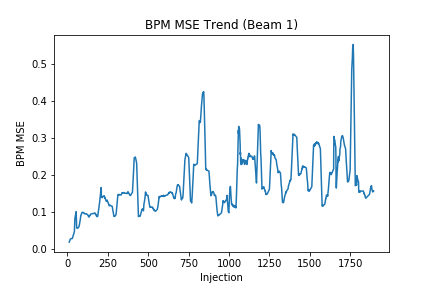
\includegraphics[width=2.5in]{BPM_MSE_Trend_B1}
		\caption[BPM MSE Trend B1]{Trend Component of the BPM MSE for Beam 1}
		\label{fig::BPM_MSE_Trend_B1}
	\end{figure}
	
	\subsection{Anomaly Detection}

	\paragraph{3D LOF}Of the  60 injections detected as anomalies by the 3D LOF algorithm for Beam 1, 39 of these were found to be actual anomalies (65\%). These detected points can be seen in Figure \ref{fig::3D_results1} where the green points represent the correctly classified injections and the red points represent the false-positives generated. Of the 98 injections detected as anomalies by the 3D LOF algorithm for Beam 2, 45 of these were found to be actual anomalies (45.91\%). As can be clearly seen in Figure \ref{fig::3D_results1}, performing LOF on this 3 dimensional dataset is not sufficient to explain the causes for anomalies as many points that are clearly outliers are not anomalous injections after all. The algorithm still performed reasonably well however and adding more dimensions might improve its performance.
	
	\begin{figure}[!t]
		\centering
		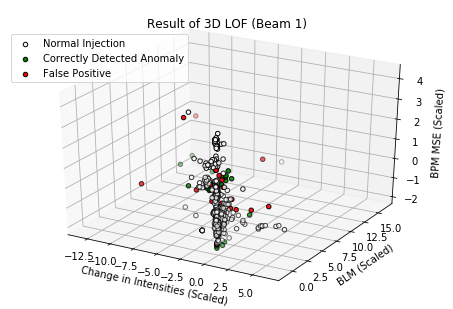
\includegraphics[width=2.5in]{3D_LOF_Results}
		\caption[3D LoF Results Beam 1]{3D Plot Highlighting Anomalies Detected by the 3D LOF Algorithm for Beam 1}
		\label{fig::3D_results1}
	\end{figure}

	\paragraph{3D DBSCAN }The DBSCAN algorithm seems to have a worse performance than the LOF algorithm for 3D data. In fact, only 40 points were detected as anomalous by this algorithm for Beam 1 and 23 (57.5\%) points were found to be actual anomalous injections. Furthermore, 60 points were detected for Beam 2 where only 28 (46.67\%) were actual anomalies. 
	
	\begin{figure}[!b]
		\centering
		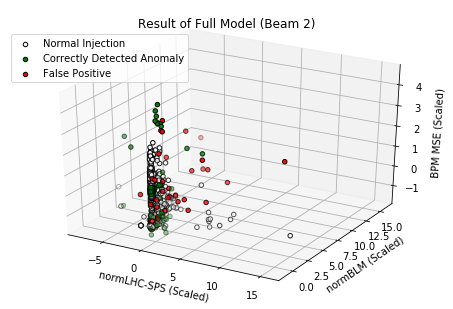
\includegraphics[width=2.5in]{Beam2_Full_Results}
		\caption[Full Dataset Results Beam 2]{3D Plot Highlighting Anomalies Detected by the Full LOF Algorithm for Beam 2}
		\label{fig::Full_results2}
	\end{figure} 
	

	\paragraph{Full Model}As expected, running LOF on the full dataset seems to have provided better results than when the 3D dataset was used. In particular, of the 64 injections detected as anomalous for Beam 1, 46 (71.88\%) of these were actual anomalies.  96 injections were detected to be anomalous for Beam 2 and 61 (63.54\%) of these were actual anomalies. Once again it can be noted from Figure \ref{fig::Full_results2} that some points which are clearly outliers for the provided dimensions are actually not anomalies. This can be seen in particular for high beam losses. There must be a parameter that's not captured in this model that's causing this phenomenon, transforming the data using PCA might thus improve the algorithm's performance.

	\paragraph{PCA Model}Although through PCA, the transformation of the data led to certain injections (such as those with high losses but still not anomalous) to not be incorrectly classified, the overall performance was similar to that of the full model. Of the 63 injections that were classified as anomalies, 43 (68.25\%) of them were actual anomalies for Beam 1. For Beam 2 however, 115 points were classified as anomalies and 65 (56.52\%) of them were actual anomalies.

	\paragraph{Nature of Anomalous Injections}One of the purposes of this study is to provide clear visual representations of the anomalies in order for experts to understand more clearly the nature of these anomalies with respect to the studied parameters. Figures \ref{fig::TrueAnomalies} and \ref{fig::TrueAnomalies2} highlight these points.
	
	\begin{figure}[!t]
		\centering
		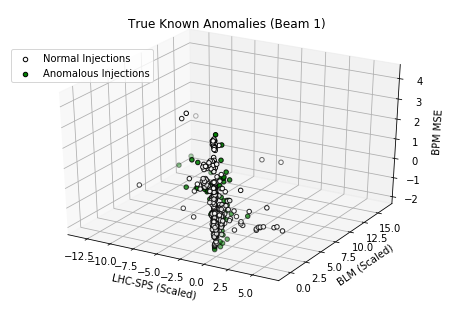
\includegraphics[width=2.5in]{TrueAnomalies}
		\caption[True Anomalous Injections (Beam 1)]{3D Plot Highlighting the Known Anomalies for Beam 1}
		\label{fig::TrueAnomalies}
	\end{figure}
	
	\begin{figure}[!t]
		\centering
		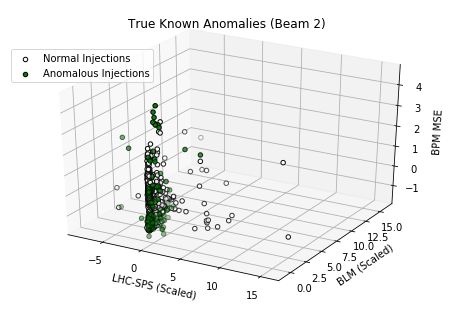
\includegraphics[width=2.5in]{Beam2_TrueAnomalies}
		\caption[True Anomalous Injections (Beam 2)]{3D Plot Highlighting the Known Anomalies for  Beam 2}
		\label{fig::TrueAnomalies2}
	\end{figure} 
	
	\section{Evaluation}
	\par The overall results for Beam 1 of all the algorithms are summarised in Table \ref{tab::Beam1_results}. Table \ref{tab::Beam1_efficiency} shows the efficiency metrics for Beam 1 and Table \ref{tab::Beam1_performance} shows the performance metrics for Beam 1. Similarly for Beam 2, the overall results are summarised in Table \ref{tab::Beam2_results}. Table \ref{tab::Beam2_efficiency} shows the efficiency metrics for Beam 2 and Table \ref{tab::Beam2_performance} shows the performance metrics for Beam 2.
	
	\begin{table}[!h]
		\renewcommand{\arraystretch}{1.3}
		\caption[Beam 1 Results]{Summary of Results for Beam 1}
		\label{tab::Beam1_results}
		\centering
		\resizebox{3.5in}{!}{
			\begin{tabular}{|l|l|l|l|l|l|}
				\hline
				\textbf{Method}     & \textbf{Total Anomalies} & \textbf{True Positives} & \textbf{True Negatives} & \textbf{False Positives} & \textbf{False Negatives} \\ \hline
				\textbf{3D LoF}     & 60                       & 39                      & 745                     & 21                       & 51                       \\ \hline
				\textbf{3D DBSCAN}  & 40                       & 23                      & 749                     & 17                       & 67                       \\ \hline
				\textbf{Full Model} & 64                       & 46                      & 748                     & 18                       & 44                       \\ \hline
				\textbf{PCA Model}  & 63                       & 43                      & 746                     & 20                       & 47                       \\ \hline
			\end{tabular}
		}
	\end{table}
	
	\begin{table}[!h]
		\renewcommand{\arraystretch}{1.3}
		\caption[Beam 1 Efficiency Metrics]{Efficiency of Algorithms for Beam 1}
		\label{tab::Beam1_efficiency}
		\centering
		\begin{tabular}{|l|l|l|l|}
			\hline
			\textbf{Method}     & \textbf{Accuracy} & \textbf{Sensitivity} & \textbf{Specificity} \\ \hline
			\textbf{3D LoF}     & 91.59\%           & 43.33\%              & 97.26\%              \\ \hline
			\textbf{3D DBSCAN}  & 90.19\%           & 25.56\%              & 97.78\%              \\ \hline
			\textbf{Full Model} & 92.76\%           & 51.11\%              & 97.65\%              \\ \hline
			\textbf{PCA Model}  & 92.17\%           & 47.78\%              & 97.39\%              \\ \hline
		\end{tabular}
	\end{table}
	
	\begin{table}[!h]
		\renewcommand{\arraystretch}{1.3}
		\caption[Beam 1 Performance Metrics]{Performance of Algorithms for Beam 1}
		\label{tab::Beam1_performance}
		\centering
		\begin{tabular}{|l|l|l|}
			\hline
			\textbf{Method}     & \textbf{Precision} & \textbf{F-measure} \\ \hline
			\textbf{3D LoF}     & 0.65               & 0.52               \\ \hline
			\textbf{3D DBSCAN}  & 0.575              & 0.3538461538       \\ \hline
			\textbf{Full Model} & 0.71875            & 0.5974025974       \\ \hline
			\textbf{PCA Model}  & 0.6825396825       & 0.5620915033       \\ \hline
		\end{tabular}
	\end{table}
	
	\begin{table}[!h]
		\renewcommand{\arraystretch}{1.3}
		\caption[Beam 2 Results]{Summary of Results for Beam 2}
		\label{tab::Beam2_results}
		\centering
		\resizebox{3.5in}{!}{
			\begin{tabular}{|l|l|l|l|l|l|}
				\hline
				\textbf{Method}     & \textbf{Total Anomalies} & \textbf{True Positives} & \textbf{True Negatives} & \textbf{False Positives} & \textbf{False Negatives} \\ \hline
				\textbf{3D LoF}     & 98                       & 45                      & 1024                    & 53                       & 89                       \\ \hline
				\textbf{3D DBSCAN}  & 60                       & 28                      & 1045                    & 32                       & 106                      \\ \hline
				\textbf{Full Model} & 96                       & 61                      & 1042                    & 35                       & 73                       \\ \hline
				\textbf{PCA Model}  & 115                      & 65                      & 1027                    & 50                       & 69                       \\ \hline
			\end{tabular}
		}
	\end{table}
	
	\begin{table}[!h]
		\renewcommand{\arraystretch}{1.3}
		\caption[Beam 2 Efficiency Metrics]{Efficiency of Algorithms for Beam 2}
		\label{tab::Beam2_efficiency}
		\centering 
		\begin{tabular}{|l|l|l|l|}
			\hline
			\textbf{Method}     & \textbf{Accuracy} & \textbf{Sensitivity} & \textbf{Specificity} \\ \hline
			\textbf{3D LoF}     & 88.27\%           & 33.58\%              & 95.08\%              \\ \hline
			\textbf{3D DBSCAN}  & 88.60\%           & 20.90\%              & 97.03\%              \\ \hline
			\textbf{Full Model} & 91.08\%           & 45.52\%              & 96.75\%              \\ \hline
			\textbf{PCA Model}  & 90.17\%           & 48.51\%              & 95.36\%              \\ \hline
		\end{tabular}
	\end{table}
	
	\begin{table}[!h]
		\renewcommand{\arraystretch}{1.3}
		\caption[Beam 2 Performance Metrics]{Performance of Algorithms for Beam 2}
		\label{tab::Beam2_performance}
		\centering
		\begin{tabular}{|l|l|l|}
			\hline
			\textbf{Method}     & \textbf{Precision} & \textbf{F-measure} \\ \hline
			\textbf{3D LoF}     & 0.4591836735       & 0.3879310345       \\ \hline
			\textbf{3D DBSCAN}  & 0.4666666667       & 0.2886597938       \\ \hline
			\textbf{Full Model} & 0.6354166667       & 0.5304347826       \\ \hline
			\textbf{PCA Model}  & 0.5652173913       & 0.5220883534       \\ \hline
		\end{tabular}
	\end{table}
	
	\par In both cases, the Full Model has outperformed all the other models, achieving the highest accuracy, precision and F-measure. An accuracy of 92.76\% and 91.08\% is quite high and is one of the positive outcomes of this study. The number of anomalies detected in beam 2 was higher than that of Beam 1, however with this increase in anomalies there seems to be a decrease in precision. It is also worth noting that the sensitivity is rather low, having a value of 51.11\% for Beam 1 and 45.52\% for Beam 2. The fact that the probability of a true anomaly being detected by the algorithm is so low means that further work still could be done to improve the overall performance. The F-measure also highlights this fact as these values are less than expected.
	
	\section{Conclusions and Future Work}

	\par In this study, LOF and DBSCAN were applied to data gathered from sensors around the moment of injection from the SPS to the LHC as unsupervised anomaly detection algorithms on various datasets. These anomalous points were then presented and it was concluded that the best performing algorithm in this case was LOF when applied to the full dataset with all the provided parameters. Furthermore, the beam displacement over time was shown and the nature of the anomalies were presented in 3D plots.
	
	\par Similar to Valentino \textit{et. al.}'s study of 2017 \cite{Valentino2017}, this proposed method can positively identify anomalous injections. However the method could use some tweaking as just like in Halilovic's thesis \cite{Halilovic2018}, the best performance still ``leaves something to be desired'' as there were still a large number of false positives being detected.
	
	\par One limitation in this study came from the loss in performance of this algorithm on the PCA Model. This could stem from the fact that when performing PCA, only 80\% of the true variance of the data was kept. It would be interesting to see if the results would improve if more principal components were kept.
	
	\par As anomaly detection in particle accelerators using unsupervised machine learning has not been explored much as of yet, further research in the area could prove to be beneficial not just for particle accelerator research but also for time series research in general. Further studies on properly fitting the parameters and their effect on the performance of the algorithms would be interesting. Also, as these techniques have the potential of detecting anomalies not being picked up by the IQC, a study on implementing such a method in real time to work in conjunction with the IQC could prove beneficial to reduce the number of anomalous injections in the LHC and save researchers time and money when running these tests. Furthermore, now that a labelled dataset was created for this study, future work on using supervised learning on this data could result in some interesting results, possibly leading to a more accurate model.
	
	\bibliographystyle{IEEEtran}
	\bibliography{biblio}

\end{document}